\documentclass[11pt]{article}
\usepackage{amsmath,amssymb}
\usepackage[utf8]{inputenc}
\usepackage{graphicx}
\usepackage{booktabs} 
\usepackage{caption}


\usepackage[margin=1in]{geometry}
\usepackage{setspace}
\doublespacing

\title{ Instability and the Economy, A Case Study: Pakistan. }
\author{ Taahaa Mir }
\date{April 2023}

\begin{document}

\maketitle

\newpage


\section{Introduction}

On April 10th 2022, Imran Khan, the 22nd Prime minister of Pakistan was ousted from power making him another prime minister that failed to complete their term as prime minister. The country’s economy now faces severe hardship following his ouster and a resulting economic crisis. The nation faces issues such unemployment with over five million people losing their jobs just through the textile industry (Pakistan Today 2020). In addition, Pakistan’s currency plunged to 287.59 Pakistani Rupees against the US dollar from 188.17 (XE) when Imran Khan was ousted. Yet, instability is something Pakistan has dealt with throughout it’s existence. Out of 22 prime ministers, neither one has ever completed a full term. Each was either ousted, assassinated, resigned, or finished a term they did not start (Vox 2018). Furthermore, Pakistan has faced three successful military coups and was ruled by the military for 36 years (IndiaToday 2022), almost half its existence. Situations such as this aren’t just limited to Pakistan, many developing nations suffer from instability and therefore it is imperative for policy makers and researchers to understand the relationship between instability and the economy. \newline

The relationship between instability and economic growth remains a widely studied topic in literature. Many factors have been identified as potential causes of instability including migration of skilled workers, political crises, fiscal mismanagement (Kerr, S., Kerr, W., Özden, C., \& Parsons, C. 2017). Further causes have been attributed to natural disasters (Ferris, E. 2010). The aim of my study is to see what role these factors play in the context of Pakistan’s economy. \newline

Therefore, my paper aims to explore the relationship between instability and Pakistan’s economy by addressing two main questions:
\begin{itemize}
    \item In the short term, how does instability impact inflation in Pakistan?
    \item How much of an impact does instability have on the People of Pakistan?
\end{itemize}

To answer these questions, we use time series data from 2012 to 2022. We employ a Lagged Multiple Regression model using the variable Inflation as the dependent variable, to capture the impact of instability on the economy but also on how it impacts people. Secondly, we use the variable EPU (Economic Policy Uncertainty Index) as a proxy variable for instability. This takes into account the various causes of instability discussed earlier. Finally, we take into account some control variables in our model. \newline

Literature based on this topic is abundant, Qureshi, Ali and Khan (2010) conducted an empirical analysis of the relationship between political instability and economic development in Pakistan. They used annual time series data from 1971-2008. The authors, by constructing a political instability index, utilized the Principle Components technique to address their question. Their finding displayed a negative relationship between political instability and economic development in Pakistan. The political instability index consisted of variables such as General Strikes, War, Government change and other variables inline with the causes of instability that we discussed earlier. This paper’s findings were supported by other papers that analyzed completely different countries. In their paper, Asteriou and Price (2000) also analyzed the impact of political uncertainty on economic growth in the UK. The authors used six political variables and analyzed their impacts on GDP growth. By utilizing time series analysis using OLS, GARCH and GARCH-M models, their findings again suggested a strong negative correlation between political instability and the growth of UK’s GDP. Pasha (2020)’s paper focused on the relationship between political instability and economic growth in Guyana. Similar to Pakistan, Guyana faces a history littered with political instability and ethnic conflict. The paper employed GARCH(1,1) models to study this relationship. The results imply that causes of instability such as changes in the heads of state has a significant positive impact on growth rates whereas other causes such as strikes has a significant negative impact. Other variables such as assassinations and riots have no significant relationship with economic growth rates. \newline

Regardless, most of the literature supports the hypothesis that instability does have a significant impact on the economy regardless of whether they are a more or less economically developed nation, and this impact is usually negative for the economy. Our research paper uses monthly time series data from 2012 to 2022 in contrast to the annual data used by the majority of other literature. Through this, the analysis will be able to capture short term fluctuations and dynamics that may be difficult to capture through annual data. Furthermore, this paper can provide insights into mechanisms through which instability affects economic growth. This would help complement the findings of literature that uses annual data. In addition, the context of Pakistan would help our analysis take unique institutional and historical factors into account resulting in a more beneficial analysis for the policy makers of Pakistan. \newline

After our analysis, our regression analysis using monthly time series data will reveal that increased lagged instability has a significant and positive effect on Inflation in Pakistan. This is inline with the majority of the literature done on this topic. However, although significant, the impact instability has on the economy is small, the results also indicate that instability in the current period doesn’t have a significant impact on inflation. This can be explained by the possibility that immediate changes resulting in instability require time to impact the economy. Moreover, the analysis uncovered significant relationships between inflation and some of the control variables such as the exchange rate. Overall, the results suggest that policy makers need to look at other factors than instability when taking into account Pakistan’s economy and inflation. 


\section{Conceptual Framework}

The conceptual framework behind this paper is embedded in the idea that instability negatively impacts Pakistan’s economy and therefore the well-being of its people. Instability can adversely affect Pakistan through a multitude of channels. First, we can look at what instability would entail for economic growth. \newline

The impact of instability on economic growth can be significant and can affect it through various means. Instability, in particular political instability, would decrease investor confidence through the resulting uncertain environment. This is true for both domestic and foreign investment, (Perotti 1996). This lack in investment can also result in a decline in productivity which further impacts negatively on economic growth. Investment is required for the acquisition of capital goods. Furthermore, it is also essential for research and development. A lack of investment would negatively impact this and therefore have a harmful effect on the economy, (McKinsey Global Institute 2021). In addition, instability may result in fiscal mismanagement, this is especially true in the case of democracies such as Pakistan. Governments may often prioritize short-term political gains during critical times such as elections or periods of instability over economic development, (Anderson, V. 2013). Pakistan has suffered from this throughout its history and the impacts of this can be seen on its long-term economic growth. Moreover, instability can result in a disruption of economic activity leading to damaging impacts for the people of the country. This may happen through inconsistent economic policies as a result of uncertainty, damaging infrastructure through strikes. Overall, poor economic policies due to uncertainty can diminish productivity, innovation and competitiveness resulting in further damage to the economy, (Shehzadi, I., Siddique, H. M. A., \& Majeed, M. T. 2019). \newline

Secondly, instability has further negative impacts than just on economic growth. Instability can hamper Human Capital Development. In unstable situations, governments face a great deal of difficulty trying to allocate resources to critical services such as education and healthcare, (Gyimah-Brempong, K., \& Munoz de Camacho, S. 1998). This lower level of education access would be extremely damaging for human capital accumulation. A further problem is posed when skilled workers migrate to seek refuge in more stable environments resulting in a “brain drain”. As a result, the country suffers from a lack of development of a stable workforce, (Pasha 2020). \newline

Thirdly, instability may also play a role when considering income inequality and poverty. While governments struggle in times of instability, they might find it difficult to, or not prioritize to, implement policies that alleviate poverty and reduce income disparity, Shehzadi, I., Siddique, H. M. A., \& Majeed, M. T. (2019). \newline

These factors makeup the conceptual framework that builds on the idea that instability has negative implications for not just the economy of Pakistan but also the well-being of its people. Pakistan can suffer as a result of a lack of investment, poor fiscal policies and a lack of human capital development. As a result, this gives us further reason to predict that our analysis would indicate a significant, positive relationship between instability and inflation. 

\section{Econometric Model}

In this section, we present the econometric model that will be used to analyze the impact of instability on inflation in Pakistan. To include instability in our model, we use a proxy variable that measures Economic Policy Uncertainty. Furthermore, we include several control variables in addition to the Economic Policy Uncertainty Index variable in our model. Through this model, the overall research question that we are aiming to answer is: “How does instability affect Pakistan’s Economy?”. \newline

To answer this question, a rigorous procedure was followed to ensure that we have an optimal model. The procedure included tests for autocorrelation, granger causality, optimal lag, tests for multicollinearity, stationary tests and optimal variable selection. \newline

We began our analysis by testing for autocorrelation. The presence of autocorrelation would render OLS an unhelpful way to estimate our model as it would violate key assumptions of the model resulting in biased and inconsistent estimates. To test for this, we inspected autocorrelation plots for each of the variables in our dataset (Figure 1). The graphs indicated the presence of autocorrelation in all variables except FDI (Figure 2). As a result, we could not use OLS without further processing our data.\newline

Given that we are conducting time series analysis, it is essential to evaluate the stationarity of the data. We do this by testing each series for a unit root through the Dickey-Fuller test. This is important to test for as non-stationary variables would result in spurious regression results. Our test results characterized several variables as being non-stationary including: Interest Rates, Imports, Exports, Consumer Confidence, Exchange Rate, Pakistan Stock Exchange Price and Inflation Rate. To mitigate this issue, we applied first differencing to each of these variables and re-ran the Dickey-Fuller tests. This time, the results showed that these variables were free from any non-stationary issues and we were allowed to proceed.\newline

After testing for autocorrelation and stationarity in our time series data, it is important to examine each variable for any time trends. We do this by graphing each variable with respect to time (from 2012 to 2022)(Figure 3) and investigating each graph for any time trends. Our graphs displayed no evidence of any time trends and we can therefore proceed.\newline

Variable selection is important in our model as we need to select variables to optimize the tradeoff between the predictive power of our model and to prevent underfitting. Firstly, we use Granger Causality tests to test which variables exhibit causal behavior on our dependent variable which is Inflation (First Differenced). These tests can help us determining which pf our variables from our dataset are statistically significant predictors of Inflation (First Differenced). If a variable is found to be a significant predictor of Inflation (First Differenced), we include this variable for consideration in our model. The variables that exhibit this behavior are: Economic Policy Uncertainty, Interest Rate (First Differenced), Imports (First Differenced), Exports (First Differenced), PKR to USD Exchange Rate (First Differenced). \newline

In addition, we need to select the optimal lag structure for our model, to do this we used the Akaike Information Criterion (AIC) to select the optimal lag structure of each variable that is remaining to be considered for our model. This was done by minimizing the AIC for each variable and including the optimal lags in our model for further consideration. The lower AIC indicates a better model fit. These variables were then regressed on Inflation (First Differenced) and to test for multicollinearity we used the variance inflation factor (VIF), which reported no evidence of multicollinearity. \newline

We then also test for heteroskedasticity using the Breusch-Pagan / Cook-Weisberg test for heteroskedasticity to observe that our model does  suffer from heteroskedasticity. The Breusch-Pagan / Cook-Weisberg test for heteroskedasticity tests for the hypothesis:
\begin{verbatim}
    H_0: Constant Variance    
\end{verbatim}
Our p-value is 0.0108, indicating that there is evidence of heteroskedasticity in our model, therefore, we will use Newey West HAC standard errors to correct this.\newline

Still, our current regression model suffers from the inclusion of many irrelevant variables (Table 1). We can see that many of these variables have p-values far greater than the threshold 0.05. Even if we raise the threshold to 0.1, we still see many variables and lags as not being significant. As a result, we choose to drop some of these irrelevant variables leaving us with the independent variables: Economic Policy Uncertainty (with no and one lag), Interest (First Difference, three lag), Imports (First Differenced, no lag, one lag, two lag), PKR USD exchange rate (two lags). The economic justification of the lag stems from the intuitive idea that impacts of changes in these lagged variables will take some time to impact inflation. This time was determined by the regression results.\newline

Before arriving at our final model, we need to test for seasonality, to do this we create 11 dummy variables representing the 11 months of the year. We include this in our regression model and carry out an F-test to determine whether the coefficients of the month variables are significant. That is, we test for:
\begin{center}
    $H_0: \beta_2 = \beta_3 = \beta_4 = \beta_5 = \beta_6 = \beta_7 = \beta_8 = \beta_9 = \beta_{10} = \beta_{11} = \beta_{12} = 0$    
\end{center}
where $\beta_2$ to $\beta_{12}$ are the coefficients of the seasonal dummies for the second to twelfth months, respectively. For this, we have a p-value of 0.9957. With this, we fail to reject the null hypothesis and we can conclude that there is no evidence of seasonality in our series. Therefore, we can drop the month variables from our model. \newline

Based on this analysis, we arrive to the following model:
\begin{center}
    $\Delta Inflation_t = \beta_0 + \beta_1EPU_t + \beta_2EPU_(t-1) + \beta_3 \Delta  Interest_{t-3} + \beta_4 \Delta  Imports_t + \beta_5 \Delta Imports_{t-1} + \beta_6 \Delta  Imports_{t-2} + \beta_7 \Delta  PKRUSD_{t-2} + \epsilon_t$  
\end{center}

where $\Delta Inflation_t$ is the change in inflation rate at time t, $EPU_t$ is the economic policy uncertainty at time t, $\Delta Interest_{t-3}$ is the difference in interest rates three periods prior, $\Delta Imports_t$ and its lags represent the changes in import volume, $\Delta PKRUSD_{t-2}$ is the change in the exchange rate (Pakistani Rupee per US Dollar) two periods prior, and $\epsilon_t$ is the error term at time $t$. The model is estimated using Newey-West standard errors to account for heteroskedasticity and autocorrelation, with a lag length of 3 periods. \newline

We also carry out a Shapiro-Walk test to ensure that the error terms produced by our regression model are normally distributed to satisfy one of the assumptions we are making. This test tests the null hypothesis that the residuals of our model are normally distributed against the alternative hypothesis that they are not. The residuals from our regression models are used in this test. Through this test, we obtain a p-value of: 0.45919 and we therefore fail to reject this null hypothesis. This implies that there is not enough evidence to suggest that our error terms are not normally distributed. \newline

The final model has been carefully selected to meet all the assumptions of the regression model and it has been thoroughly tested. This provides a reliable framework for making policy-relevant decisions. By investigating the coefficients of the variables, we will be able to assess the impact in terms of magnitude and direction that each of our variables has on Inflation. In our case, the most relevant variable is economic policy uncertainty. With these results, we can contribute to understanding how instability through economic policy uncertainty impacts Pakistan’s economy and its people through the lens of inflation.

\section{Data}
The variables used in our analysis are listed in Table 2 with their descriptions and sources. Not all of these variables ended up being used in our model. In this section, we will only discuss the important variables that were used in our model. \newline

In our dataset, the most important variable in the context of our research question is Economic Policy Uncertainty (EPU) Index as this is being used as the proxy variable for Instability as an explanatory variable. The data for this variable was obtained through the Policy Uncertainty website and was developed by Baker, Bloom and Davis (2016). This index is based on a text analysis of articles from major newspapers in the context of each country. Using this, the index assigns values based between 0 to 500 representing the degree of uncertainty expressed in news articles regarding economic policy decisions in each country. Higher values indicate that there is a greater degree of economic policy uncertainty. In our study, higher EPU index values can reflect a higher degree of instability often through uncertain economic policy decisions that governments make during unstable periods. The summary statistics for this variable are displayed in Table 3, its variation overtime is displayed in Figure 4. \newline

Another important variable in our analysis is the Inflation rate, its summary statistics are displayed in Table 4. This captures the increase in the general price level of goods and services in the economy, making it the perfect variable to capture the impacts of Instability on not just Pakistan’s economy but also its people. Higher levels of inflation would indicate a greater deal of suffering for the people of Pakistan while also indicating the poor health of Pakistan’s economy. The inflation rate that we obtained is from the Pakistan Bureau of Statistics and is in percent. Note that in our analysis we discovered that this series was non-stationary, as a result, we had to apply first differencing to this variable. The summary statistics due to this change are displayed in Table 5. The variation of Inflation (First Differenced) overtime is displayed in Figure 5. \newline

The remaining variables in our model are three control variables: Interest Rate (Interest), Imports (Imports) and USD to PKR exchange rate (PKRUSD). The summary statistics for these are in Table 6. The data for Interest Rates was collected from the State Bank of Pakistan while the data for Imports and the exchange rate came from Pakistan Bureau of Statistics and Investing.com respectively. The imports variable is a useful variable to include as a control variable as it can act as a proxy for international trade and economic activity in the context of Pakistan. Furthermore, the exchange rate reflects the strength of Pakistan’s economy and currency and is therefore another good control variable to include in our model. Finally, the interest rate is a tool used to manage inflation and should therefore be included as a control variable. By including these variables as control variables, we account for their potential influence on the dependent variable, Inflation. Through this, we can isolate the impact that instability has on inflation rate and determine the precise relationship between instability and inflation. These series were also shown to be non-stationary and therefore, first differencing was applied to each of these control variables. The updated summary statistics are displayed in Table 7.

\section{Results}
By estimating our lagged multiple regression model using Newey-West HAC standard errors, we obtain the regression results displayed in Table 8. These results provide insight into the relationship between instability, measured through the proxy variable EPU, and inflation. As a result, the coefficient of EPU, it’s magnitude and it’s statistical significance would serve as useful information for policy makers and other researchers in understanding the impacts that instability can have on inflation and therefore, it’s people and the economy. \newline

The main variable in our analysis is EPU as it models instability, therefore we can investigate the coefficient of this variable. Looking at the contemporaneous result, we see that the coefficient is negative (-0.0032504) indicating a decrease in the inflation rate (first difference) as EPU increases. This is certainly a surprising result considering our discussion in the Conceptual Framework section of our paper, yet this can be easily explained by examining the magnitude and the statistical significance of the coefficient. Firstly, the magnitude of contemporaneous EPU is very small, even a 100-point increase in EPU (which is drastic considering the range is between 0-500) would only decrease the difference in interest rates by 0.3\%. Knowing that the interest rate (first difference) has a range from -4.08\% to 7.52\% (Table 5), this is a very small change. Moreover, looking at the statistical significance of this coefficient, we notice that it has a p-value of 0.222 which is far greater than our threshold of 0.05. Therefore, we can conclude that there is no evidence that contemporaneous EPU has any significant impact on the first-differenced inflation rate. Intuitively, this can be explained by the fact that it takes a certain amount of time for instability to be reflected in the change in interest rates over time. This can be confirmed when we investigate the coefficient of the lagged EPU. \newline

The coefficient of the lagged EPU index indicates that a 100-unit increase (which is a significant increase) in the EPU index in the previous period leads to a 0.9\% increase in the difference between inflation rates. Again, looking at the range of the first differenced inflation rate, although this has a larger impact than the EPU index that is not lagged, the magnitude is still small. By investigating the statistical significance of this coefficient, we see that it has a p-value of 0.019 and is therefore statistically significant. The sign of the coefficient is what we expected in our conceptual framework section of this paper. An increase in instability results in worsening inflation. Yet, it is surprising to see that the impact of instability is not as large as predicted. \newline

Our analysis consisted of robust checks and thorough tests yet there are some limitations present within our model. The first limitation being that the EPU index, although used widely for empirical analysis in the context of instability, may not capture all aspects of instability in Pakistan’s economy. It may leave out events such as regime shifts. Furthermore, our model assumes a linear relationship between the variables which may not always be the case. It is possible that the explanatory variables have a more complex relationship with the dependent variable. \newline

Despite these limitations, the model does provide some valuable insights into the relationship between instability and Pakistan’s economic health in the form of inflation. These findings can help policy makers make decisions when considering Pakistan’s economy while also inspire and guide future research on this topic.

\section{Conclusion}

This paper aimed to investigate the relationship between instability and it’s impact on the people of Pakistan as well as Pakistan’s economy. Our objective was to provide key and helpful insights into this topic for policymakers and researchers. We also aimed to make a meaningful contribution to existing literature on this topic. We predicted that instability would have a significant and negative impact on Pakistan’s economy and it’s people. Our paper asked two questions at the beginning of our analysis, these were:
\begin{itemize}
    \item In the short term, how does instability impact inflation in Pakistan?
    \item How much of an impact does instability have on the People of Pakistan?
\end{itemize}

To address these questions, we employed the Economic Policy Uncertainty Index as a proxy variable for instability. We used the Inflation Rate as the dependent variable to indicate not only the health of the economy but also the impact of the economy on the people of Pakistan. Our analysis involved a lagged multiple regression model, utilizing the Newey-West HAC standard errors to account for serial correlation and heteroskedasticity. Through the results, we were able to analyze the impact of instability as measured by EPU on the difference in inflation rate. \newline

Our findings revealed several key insights in the context of instability and its impact on the difference in inflation. First, we noted that the contemporaneous EPU index was found to have an insignificant impact on the first-differenced inflation rate. This suggests that instability has no immediate impact on inflation. We can attribute this fact to the time required for an event leading to instability to have an impact on Pakistan’s economy. However, looking at the coefficient of the lagged EPU index, it demonstrates a statistically significant and positive relationship with the difference in inflation rate which is inline with our predictions from earlier. This supports the hypothesis that there is a delayed but positive effect of instability on inflation in Pakistan. \newline

Yet, looking at the magnitude of this coefficient, we noticed that this effect was limited and smaller than anticipated. This indicates that perhaps the influence that instability has on Pakistan’s economy is not as significant as initially assumed. This would imply that perhaps there are other factors that play a much greater role in affecting the inflation rate in Pakistan than simply Instability. The results nevertheless show that it is worth promoting stability in Pakistan as it does still have some impact on inflation. \newline

Despite the thorough analysis and robust tests, our model did face certain limitations, in particular, the EPU index may not capture all aspects of instability in Pakistan, which may leave some key events out of the analysis. Furthermore, our model’s assumption of a linear relationship between the variables may result in inaccurate results if this is not the true relationship between the variables. Yet, this model is still statistically significant and does provide some valuable insight into the topic. \newline

In light of our findings, policymakers in Pakistan would be encouraged to promote stability in Pakistan, however it may be more important for the policy makers to investigate other factors that may affect inflation in Pakistan as they may have more of an impact than instability does. At the same time, future research should investigate alternative measures of instability and make use of more complex models to better understand the impact of instability on inflation in Pakistan. Such research could build a more comprehensive understanding of the factors that impact Pakistan’s economy. \newline

In conclusion, this paper has shed light on how instability has impacted the Pakistani people and Pakistan’s economy in the short run. We used the EPU index to model instability and used inflation to measure Pakistan’s economy’s health. Our finding would provide valuable insights for policy makers, guiding them towards more effective policy decisions while at the same time inspiring future research into this topic.


\section{Bibliography}
“Textile Producers Union Announces Nationwide Closure.” Pakistan Today, October 5, 2022. https://www.pakistantoday.com.pk/2022/10/05/textile-producers-union-announces-nationwide-closure/. \newline

“XE Currency Charts: USD to PKR.” XE. Accessed April 6th 2023. \newline https://www.xe.com/currencycharts/?from=USD\&to=PKR. \newline

Vox. “How Pakistan's cricket superstar became prime minister.” YouTube video, 6:00. August 29, 2018. https://www.youtube.com/watch?v=BE9kOlBRHok\&ab\_channel=Vox. \newline

“Allah, Army and America: Who Dictates Pakistan’s Politics?” Times of India, April 17th, 2022. https://timesofindia.indiatimes.com/world/pakistan/allah-army-and-america-who-dictates-pakistans-politics/articleshow/90781981.cms. \newline

Kerr, Sari Pekkala, William Kerr, Çağlar Özden, and Christopher Parsons. “Global Talent Flows.” Journal of Economic Perspectives 30, no. 4 (2016): 83-106. https://blogs.worldbank.org/developmenttalk/global-talent-flows-causes-and-consequences-high-skilled-migration. \newline

Ferris, Elizabeth. “Natural Disasters, Conflict, and Human Rights: Tracing the Connections.” Brookings Institution, March 3, 2010. https://www.brookings.edu/on-the-record/natural-disasters-conflict-and-human-rights-tracing-the-connections/. \newline

Khan, Qureshi Ali. “Political Instability and Economic Development: Pakistan Time-Series Analysis.” ResearchGate (2010). https://www.researchgate.net/publication/268343329. \newline

Asteriou, Dimitrios, and Simon Price. “Political Uncertainty and Economic Growth: UK Time Series Evidence.” Scottish Journal of Political Economy 50, no. 1 (2000): 1-16. \newline

Pasha, Sukrishnalall. “The impact of political instability on economic growth: the case of Guyana” Munich Personal RePEc Archive (2020). \newline
https://mpra.ub.uni-muenchen.de/103145/1/MPRA\_paper\_103145.pdf. \newline

Perotti, Roberto, and Alesina, Alberto . “Income Distribution, Political Instability, and Investment” National Bureau of Economic Research Working Paper No. 4486 (1993). \newline https://www.nber.org/papers/w4486. \newline

McKinsey Global Institute. “Will Productivity and Growth Return After the COVID-19 Crisis?” McKinsey \& Company (2021). https://www.mckinsey.com/industries/public-and-social-sector/our-insights/will-productivity-and-growth-return-after-the-covid-19-crisis. \newline

Shehzadi, Humaira et al., “Impact of Political Instability on Economic Growth Poverty and Income Inequality.” ResearchGate (2019). \newline https://www.researchgate.net/publication/333811787\_IMPACT\_OF\newline\_POLITICAL\_INSTABILITY\_ON\_ECONOMIC\_GROWTH\_POVERTY\_AND\_INCOME\_INEQUALITY. \newline

Anderson, Vicky et al., “Politics \& Short-termism.” Intergenerational Foundation (2013). \newline https://www.if.org.uk/wp-content/uploads/2013/08/2.Politics\_\_Short-termism.pdf. \newline

Gyimah-Brempong, Kwabena and Samaria Munoz de Camacho. “Corruption, Growth, and Income Distribution: Are There Regional Differences?” Economics of Governance 3 (1998): 221–240. https://www.jstor.org/stable/4192803 \newline

Variables: KSEPrice, PKRUSD Investing.com. Accessed [April 6th 2023]. https://www.investing.com/.
Variables: FDI, Interest, IndustrialProd, ConsumerConfidence, State Bank of Pakistan. Accessed April 6th 2023. http://www.sbp.org.pk/. \newline

Variables: Imports, Exports, Inflation, Pakistan Bureau of Statistics. Accessed [April 6th 2023]. http://www.pbs.gov.pk/. \newline

Variables: EPU, Economic Policy Uncertainty. Accessed April 6th 2023. http://www.policyuncertainty.com/.

\section{Appendix}

\begin{figure}[h]
    \centering
    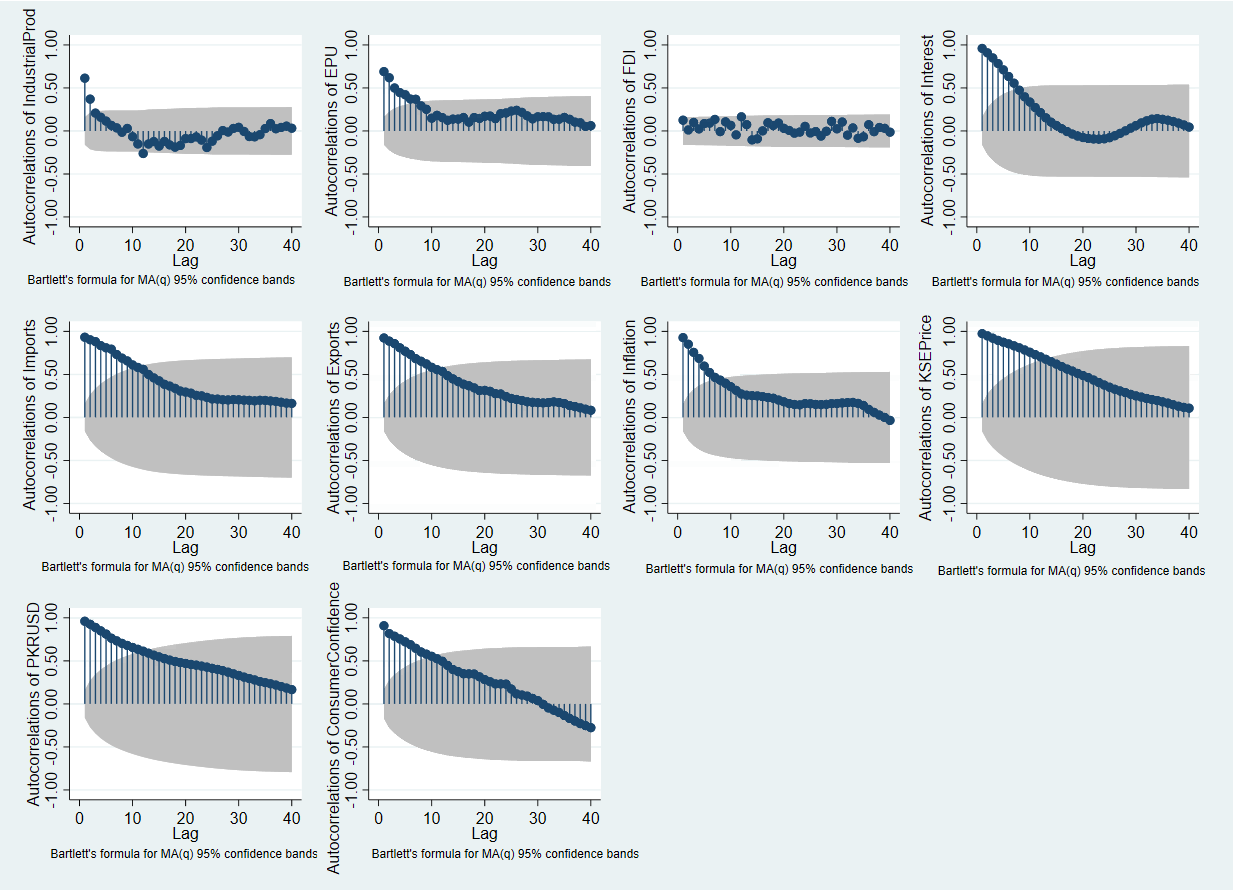
\includegraphics[width=0.8\textwidth]{images/Figure1a.png}
    \caption{Autocorrelation Plots of Variables}
\end{figure}

\begin{figure}[h]
\centering
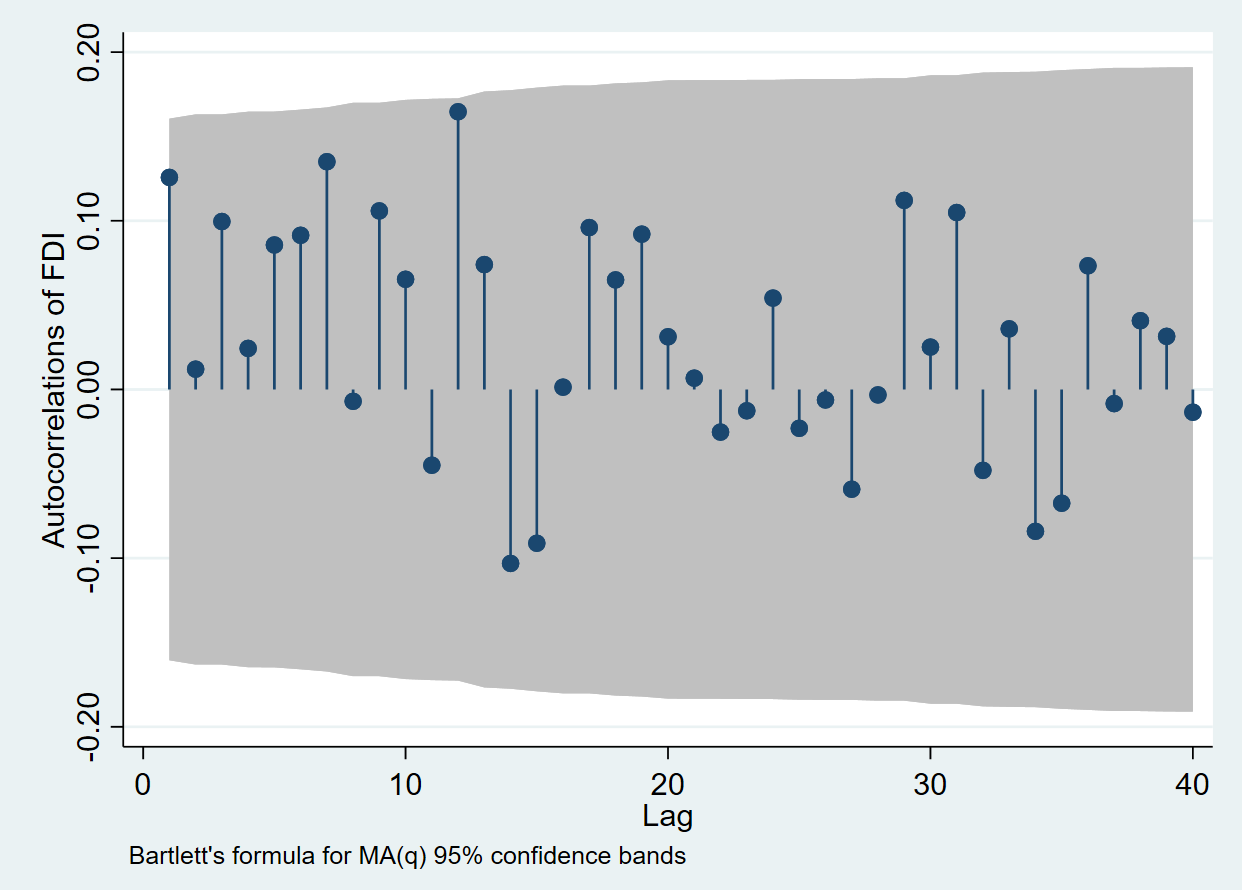
\includegraphics[width=0.8\textwidth]{images/Figure1b.png}
\caption{Autocorrelation Plot of FDI}
\end{figure}

\begin{figure}[h]
\centering
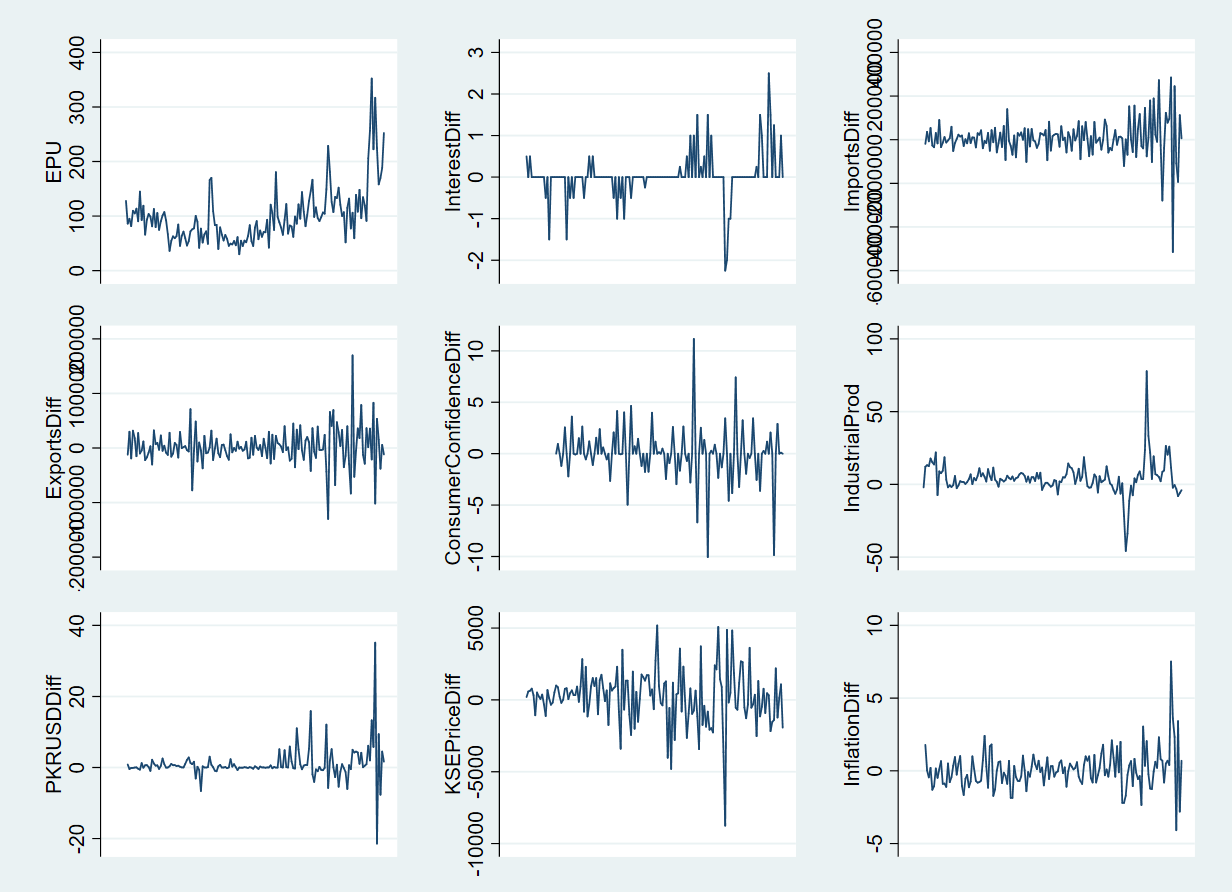
\includegraphics[width=0.8\textwidth]{images/Figure2.png}
\caption{Variable Plot Against Time}
\end{figure}

\begin{table}[ht]
\centering
\begin{tabular}{lcc}
\hline
 & Coef. & Std. Err. \\ 
\hline
\textbf{EPU} & & \\
-- & -0.0044 & 0.0033 \\
L1 & 0.0066 & 0.0029 \\
L2 & 0.0008 & 0.0044 \\
L3 & 0.0024 & 0.0040 \\
\textbf{InterestDiff} & & \\
-- & 0.1141 & 0.2812 \\
L1 & 0.0179 & 0.1863 \\
L2 & 0.5449 & 0.3422 \\
L3 & 0.5073 & 0.2909 \\
L4 & -0.4042 & 0.2607 \\
\textbf{ImportsDiff} & & \\
-- & 3.69e-06 & 2.21e-06 \\
L1 & 3.75e-06 & 2.04e-06 \\
L2 & 3.81e-06 & 2.95e-06 \\
L3 & -2.42e-06 & 1.44e-06 \\
\textbf{ExportsDiff} & & \\
-- & -7.29e-07 & 4.35e-06 \\
L1 & -5.12e-06 & 4.09e-06 \\
L2 & -3.04e-07 & 3.65e-06 \\
\textbf{PKRUSDDiff} & -0.0000 & 0.0311 \\
\textbf{\_cons} & -0.4925 & 0.2793 \\
\hline
\end{tabular}
\caption{Regression with Newey-West standard errors (rounded to two decimal places)}
\label{table:results_rounded}
\end{table}

\begin{table}[ht]
\centering
\begin{tabular}{ll}
\hline
Variable Name   & Variable Description \\
\hline
Date            & Date YMD \\
EPU             & Economic Policy Uncertainty Index\\
FDI             & Foreign Direct Investment USD Million \\
Interest        & Interest Rate in \% \\
Imports         & Imports PKR Million\\
Exports         & Exports PKR Million \\
Inflation       & Inflation in \% \\
IndustrialProd  & Change in Industrial Production in \% \\
KSEPrice        & KSEPrice in Pakistani Rupees\\
PKRUSD          & PKRUSD in Pakistani Rupees\\
ConsumerConfidence & Consumer Confidence in points.\\
\hline
\end{tabular}
\caption{Variable Names and Variable Labels}
\label{table:variables}
\end{table}

\begin{table}[ht]
\centering
\begin{tabular}{lrrrrr}
\hline
Variable & Obs & Mean & Std. Dev. & Min & Max \\
\hline
EPU & 144 & 99.99 & 52.28 & 30.06 & 352.24 \\
\hline
\end{tabular}
\caption{Summary Statistics for EPU}
\label{table:summary_statistics}
\end{table}



\begin{figure}[h]
\centering
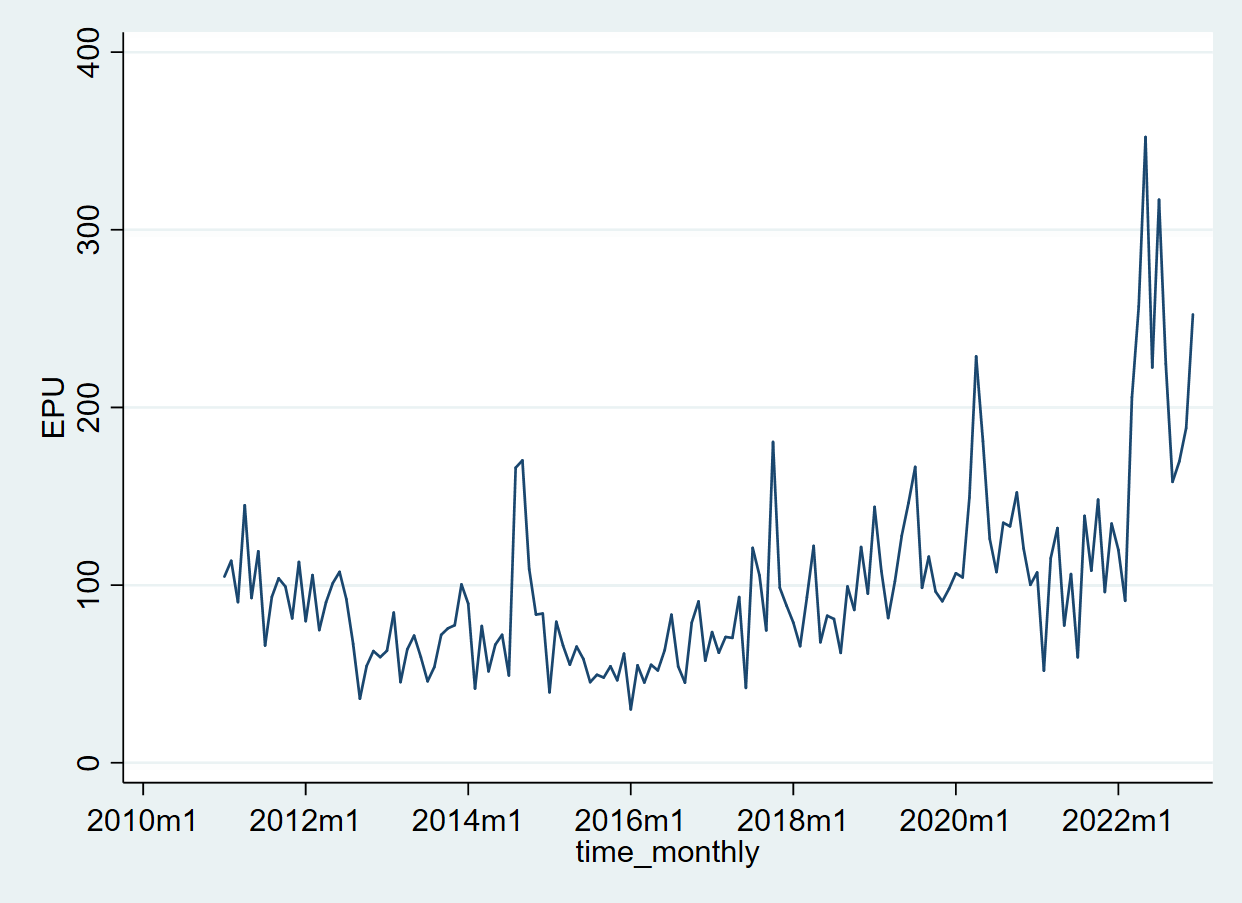
\includegraphics[width=0.8\textwidth]{images/Figure4.png}
\caption{EPU Plot Against Time}
\end{figure}

\begin{table}[ht]
\centering
\begin{tabular}{lrrrrr}
\hline
Variable & Obs & Mean & Std. Dev. & Min & Max \\
\hline
Inflation & 144 & 8.41 & 4.89 & 1.32 & 27.26 \\
\hline
\end{tabular}
\caption{Summary Statistics for Inflation}
\label{table:inflation_summary_statistics}
\end{table}

\begin{table}[ht]
\centering
\begin{tabular}{lrrrrr}
\hline
Variable & Obs & Mean & Std. Dev. & Min & Max \\
\hline
InflationDif & 144 & 0.06 & 1.30 & -4.08 & 7.52 \\
\hline
\end{tabular}
\caption{Summary Statistics for InflationDif}
\label{table:inflationdif_summary_statistics}
\end{table}


\begin{figure}[h]
\centering
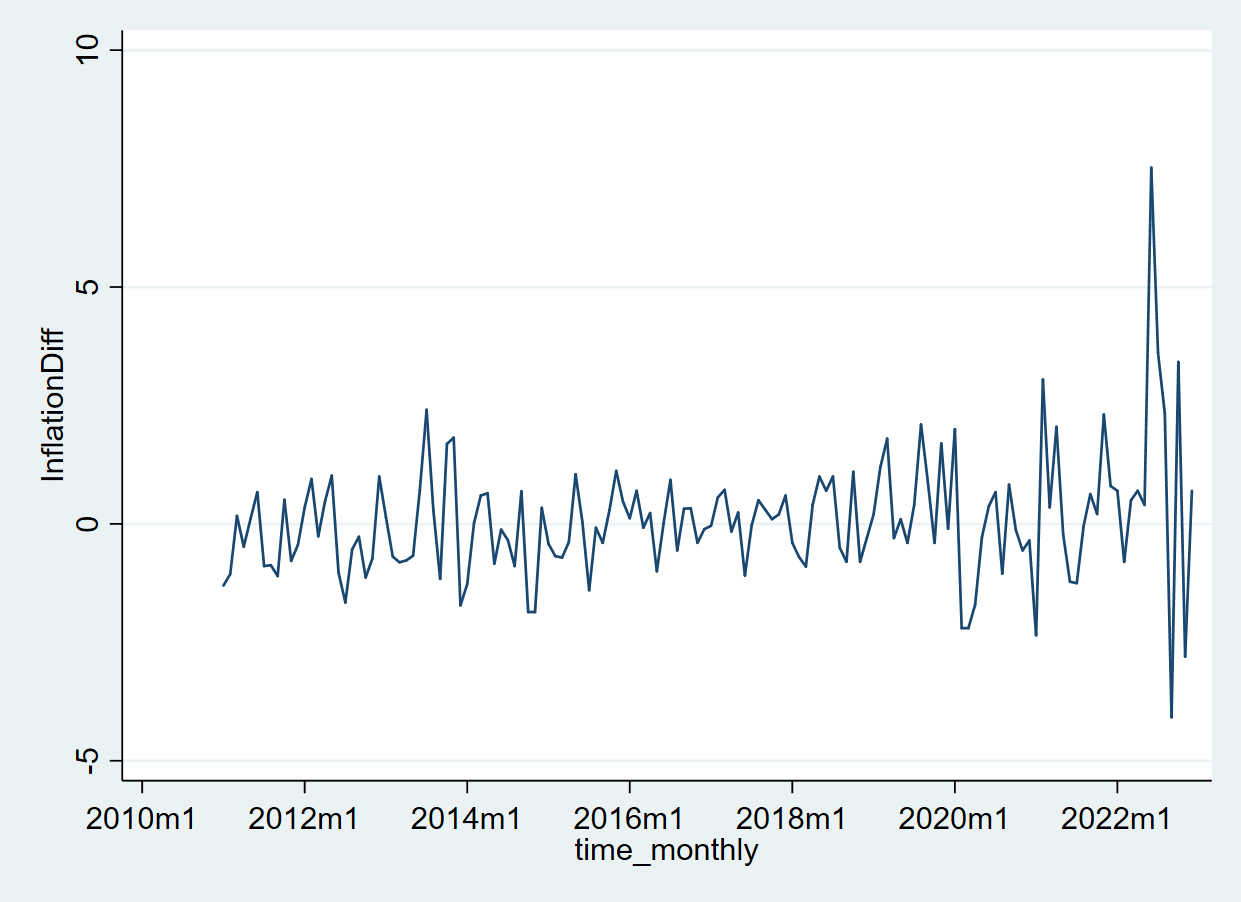
\includegraphics[width=0.8\textwidth]{images/Figure5.png}
\caption{InflationDiff Plot Against Time}
\end{figure}

\begin{table}[ht]
\centering
\begin{tabular}{lrrrrr}
\hline
Variable & Obs & Mean & Std. Dev. & Min & Max \\
\hline
Interest & 144 & 9.11 & 2.84 & 5.75 & 16.00 \\
Imports & 144 & 565215.20 & 276950.30 & 260500.10 & 1610327.00 \\
PKRUSD & 144 & 125.04 & 36.32 & 84.70 & 239.66 \\
\hline
\end{tabular}
\caption{Summary Statistics for Interest, Imports, and PKRUSD}
\label{table:interest_imports_pkrusd_summary_statistics}
\end{table}

\begin{table}[ht]
\centering
\begin{tabular}{lrrrrr}
\hline
Variable & Obs & Mean & Std. Dev. & Min & Max \\
\hline
InterestDiff & 144 & 0.02 & 0.54 & -2.25 & 2.50 \\
ImportsDiff & 144 & 5811.30 & 86490.06 & -514597.00 & 285326.00 \\
PKRUSDDiff & 144 & 0.98 & 4.60 & -21.41 & 35.16 \\
\hline
\end{tabular}
\caption{Summary Statistics for InterestDiff, ImportsDiff, and PKRUSDDiff}
\label{table:interestdiff_importsdiff_pkrusddiff_summary_statistics}
\end{table}


\begin{table}[ht]
\centering
\begin{tabular}{lcc}
\hline
 & Coef. & Std. Err. \\ 
\hline
\textbf{EPU} & & \\
-- & -0.0033 & 0.0026 \\
L1 & 0.0095 & 0.0040 \\
\textbf{InterestDiff} & & \\
L3 & 0.5911 & 0.2076 \\
\textbf{ImportsDiff} & & \\
-- & 2.96e-06 & 1.41e-06 \\
L1 & 4.18e-06 & 1.92e-06 \\
L2 & 4.67e-06 & 1.55e-06 \\
\textbf{PKRUSDDiff} & & \\
L2 & -0.0600 & 0.0261 \\
\textbf{\_cons} & -0.5465 & 0.2688 \\
\hline
\end{tabular}
\caption{Regression with Newey-West standard errors (rounded to two decimal places)}
\label{table:results_rounded}
\end{table}


\end{document}
